\documentclass[11 pt]{beamer}
\let\Tiny=\tiny

\usepackage{mathtools}
\usepackage{amsfonts}
\usepackage{amsmath}
\usepackage{graphicx}
\usepackage{pgfpages}
\usepackage[]{xcolor}
\usepackage{tikz}
\usepackage{subcaption}
\usepackage{float}

\newcommand{\meo}[1]{\texttt{#1}} % My Eyes Only: notes just for me
\newcommand{\bigo}{\mathcal{O}}
\newcommand{\extra}[1]{{\color{purple} {#1}}}

\usetheme{default}
\usecolortheme{beaver}
\usefonttheme{serif}


\beamertemplatenavigationsymbolsempty
\setbeameroption{show notes}


\newif\ifpresstime
	\presstimefalse
	% \presstimetrue

\mode<presentation>{
	\setbeameroption{hide notes}
}
\mode<handout>{
	\setbeameroption{show notes}
	\pgfpagesuselayout{2 on 1}[letterpaper, border shrink=5mm]

}


\ifpresstime
		\renewcommand{\meo}[1]{}
		\date{April 13, 2018}
		\setbeameroption{hide notes}
	\else
		\setbeameroption{show notes}
		% \setbeameroption{show only notes}
		\date{\today}
	\fi

\usetikzlibrary{arrows, automata, shapes}
\tikzset{
		initial text = {\scriptsize{\textsc{start}}},
		initial distance = 1 pt,
		every initial by arrow/.style={->},
		initial below,
		elliptic state/.style={draw,rounded rectangle},
		accepting/.style ={thick, double}
	}


\title{Kleene's Theorem}
\author{James McFeeters}
\institute {Beloit College}
\begin{document}

\frame{
	\titlepage
}

\begin{frame}
	\frametitle{Basic Definitions}
	\begin{itemize}
		\item Symbol
		\pause
		\item Alphabet ($\Sigma$)
		\pause
		\item String / word
		\begin{itemize}
			\pause
			\item The empty string ($\lambda$)
			\pause
			\item $|\lambda| = 0$
		\end{itemize}
		\pause
		\item Language
		\begin{itemize}
			\pause
			\item $\Sigma^*$: all words over $\Sigma$.
			\pause
			\item $\emptyset$
		\end{itemize}
	\end{itemize}
\end{frame}
\note{
	\textbf{Symbol:} The most basic unit of formal language theory --- like a letter in an alphabet.
	Can't be decomposed into anything and nothing can be combined into a symbol.

	\textbf{Alphabet:} A restricted set of symbols.
	Like the Latin alphabet for English or 0 and 1 for binary.
	We always assume that alphabets are nonempty and finite.

	\textbf{String:} or Word, a sequence of symbols.
	A string made entirely of symbols of one alphabet is called a string \textbf{over} that alphabet.
	We assume that strings are finite, but we don't assume that they are nonempty.
	\textbf{The Empty String:} Contains no symbols, is the string of length 0.
	Lambda is considered a string over any alphabet.
}
\note{
	\textbf{Language:} A set of strings. 
	For example, the set of all strings over an alphabet.
	The empty set is the language of NO strings over an alphabet.
	We could also just specify all the members of a language (like a dictionary).
	We're more interested in languages that are formed according to some rules so that we can describe the language without specifying all its members.
	We'll be dealing with the \textbf{regular languages}, which are formed using three set operations.
}


\begin{frame}
	\frametitle{Regular Operations}
	\begin{itemize}
		\item Union
		\item Concatenation
		\item Kleene Closure
	\end{itemize}
\end{frame}
\note{
	\textbf{Union:} probably familiar to everyone, all the strings from either language.

	Concatenation and Kleene Closure I need to define.

}


\begin{frame}
	\frametitle{Concatenation}
	\begin{columns}[T]
		\column{0.3\textwidth}
			\begin{block}{Strings}
				\begin{flalign*}
					w_1 &= ab &\\
					w_2 &= bc &\\
					w_1 w_2 &= abbc &\\
				\end{flalign*}
			\end{block}
		\column{0.5\textwidth}
		\pause
			\begin{block}{Languages}
				\begin{flalign*}
					AB &= \{ ab \mid a \in A, \, b \in B \} &\\
				\end{flalign*}
			\end{block}
	\end{columns}
	\begin{columns}[T]
		\column{0.3\textwidth}
		\pause
			\begin{flalign*}
				w^0 &= \lambda 		& \\
				w^1 &= w 			& \\
				w^2 &= ww			& \\
				w^k &= w w^{k-1} 	&
			\end{flalign*}
		\column{0.5\textwidth}
		\pause
			\begin{flalign*}
				A^0 &= \{ \lambda\} 					& \\
				A^1 &= A \{ \lambda \} = A 				& \\
				A^2 &= AA = \{ xy \mid x, y \in A \}	& \\
				A^k &= A A^{k-1}
			\end{flalign*}
	\end{columns}
\end{frame}
\note{
	Start with concatenation of strings --- just bolting one string onto the end of the other: ``run'' and ``way'' to get runway.\\[2 ex]

	For languages, we use the set product.
	The concatenation of two languages is the language of words from the first language concatenated with words of the second language.\\[2 ex]

	Next I want to go over a bit of notation that will make the Kleene Closure easier to understand.\\[2 ex]

	We use superscripts to denote concatenating a word with itself, or repeating the word some number of times.
	So repeating a word zero times gets us the empty string.\\[2 ex]

	The same is true for languages. 
	But note that repeating a language $n$ times doesn't get us all the strings in that language repeated $n$ times, it gets us any combination of $n$ words from that language.

}

\begin{frame}
	\frametitle{Kleene Closure}
	$A^*$: the \textbf{Kleene closure} of $A$.
	\pause
	\begin{align*}
		A^* &= \bigcup_{k \geq 0} A^k \\
		&= \{ \lambda \} \cup A \cup A^2 \cdots \\
	\end{align*}
	\pause
	If $A = \{ w \}$ then $A^* = \{ \lambda, \: w, \: ww, \: www, \: \dots\}$.
\end{frame}
\note{
	The Kleene closure of a language is that language repeated any number of times.\\[2 ex]

	If you have a language of just one word, you get the empty string, or that word repeated any number of times.

}

\begin{frame}
	\frametitle{Regular Languages}

	The \textbf{atomic} regular languages over an alphabet $\Sigma$ are
	\pause
	\begin{itemize}
		\item $\emptyset$
		\item $\{ \lambda \}$
		\item $\{ a \}$ for any $a \in \Sigma$ 
	\end{itemize}~\\[1 em]
	\pause

	If $A$ and $B$ are regular languages, then so are
	\begin{itemize}
		\item $A \cup B$
		\item $AB$
		\item $A^*$
	\end{itemize}
\end{frame}
\note{
	The \textbf{atomic} regular languages are the regular languages over any arbitrary alphabet.
	They are the basis for all other regular languages.
	The language containing no strings.
	The language containing just the empty string.
	The language containing a one-symbol string for each symbol in the alphabet. \\[2 ex]

	And if $A$ and $B$ are regular languages, then so are their union, concatenation, and Kleene Closure.
}

\begin{frame}
	\frametitle{Regular Expressions}

	\pause
	Atomic regular expressions:
	\begin{itemize}
		\item $\emptyset$ means $\emptyset$
		\item $\lambda$ means $\{ \lambda \}$;
		\item $a$ means $\{ a \}$ for any $a \in \Sigma$.
	\end{itemize}~\\[1 ex]
	\pause
	If $\alpha$ means $A$ and $\beta$ means $B$, then
	\begin{itemize}
		\item $\alpha \beta$ means $AB$;
		\item $\alpha + \beta$ means $A \cup B$;
		\item $\alpha^*$ means $A^*$.
	\end{itemize}
	\pause
	
\end{frame}
\note{
	Now we're going to go over two ways of representing regular languages.\\[2 ex]

	The first is \textbf{regular expressions}, which look almost exactly the same as the set notation we just used.
	The only differences are, we drop some braces, and use a plus instead of the union symbol. \\[ 2 ex]

	The actual difference is that regular expressions are a shorthand for regular languages so they aren't languages themselves, they're statements about languages.
	Two regular expressions are considered distinct, even if the languages they describe are exactly the same.\\[2 ex]

	The next way of representing regular languages is will probably seem more different.
}

\begin{frame}{Regular Expressions}
	\begin{exampleblock}{What's new here?}
	Languages:
	\[
		A^* \cup \{ \lambda \} = A^*
	\]
	\pause
	Expressions:
	\[
		\alpha^* + \lambda \neq \alpha^*
	\]
	\end{exampleblock}

\end{frame}

\begin{frame}
	\frametitle{Finite Automata}

	5-tuple: $M = (Q, \Sigma, s, \delta, F)$

	\begin{itemize}
		\pause
		\item [$Q$] the set of possible states. (Typically $q_1, q_2, \dots$.)
		\pause
		\item [$\Sigma$] the alphabet of input symbols.
		\pause
		\item [$s$] the initial state, $s \in Q$.
		\pause
		\item [$\delta$] the transition function:
		\pause
		\[
			\delta: (Q \times \Sigma) \to Q.
		\]
		\pause
		\item [$F$] the set of accepting states, $F \subseteq Q$.
	\end{itemize}
\end{frame}
\note{
	A \textbf{Finite automaton} is a machine with five parts.
	It has a finite number of configurations, which we call states.
	It moves between states when it receives an input symbol.
	Elevator example.
	We deal with machines that either accept or reject a string of inputs, based on the state of the machine after the input string.
	\begin{itemize}
		\item $Q$ is a set of states, really a set of names for states.
		These names are basically meaningless, typically they're just numbered.
		\item $\Sigma$ is the set of possible input symbols.
		\item $s$ is the state the machine starts in, before reading any input.
		\item $\delta$ tells the machine which state it should move to, given the current state and an input symbol, it outputs the next state.
		\item $F$ is all the states in which the machine is accepting the current input. Also sometimes called final states.
	\end{itemize}
}




\begin{frame}
	\frametitle{Building a Finite Automaton}
	\begin{center}
	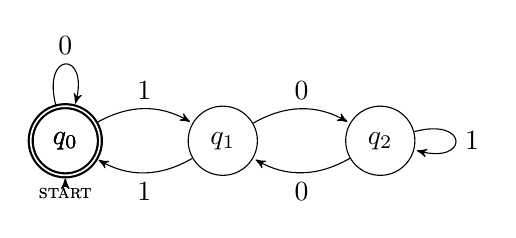
\begin{tikzpicture}[>=stealth',shorten >=1pt,auto,node distance=2cm]
		\pause % 1
		\temporal<3>
		{\node[state] (q0)                     {$q_0$};}
		{\node[state, initial] (q0)            {$q_0$};}
		{\node[state, initial, accepting] (q0) {$q_0$};}
		\node[state]                   (q1) [right of = q0] {$q_1$};
		\node[state]                   (q2) [right of = q1] {$q_2$};
		\pause % 2 Plain q0
		\pause % 3 Initial q0
		\pause % 4 Accepting q0
		\pause % 5 Show Sigma
		\path[->] (q0) edge [loop above] node {0} (q0);
		\pause % 6
		\path[->] (q0) edge [bend left]  node {1} (q1);
		\pause % 7
		\path[->] (q1) edge [bend left]  node {0} (q2);
		\pause % 8
		\path[->] (q1) edge [bend left]  node {1} (q0);
		\pause % 9
		\path[->] (q2) edge [bend left]  node {0} (q1);
		\pause % 10
		\path[->] (q2) edge [loop right] node {1} (q2);
	\end{tikzpicture}
	\end{center}
	\visible<2->{$Q = \{ q_0, q_1, q_2 \}$}\\
	\visible<3->{$s = q_0$}\\
	\visible<4->{$F = \{ q_0 \}$}\\
	\visible<5->{$\Sigma = \{ 0, 1 \}$}

\end{frame}
\note[itemize]{
	\item Build a finite automaton to accept binary numbers divisible by 3. (reading from the most significant bit).
	\item One state per possible value mod 3
	\item We start at 0, 
	\item We accept strings divisible by 3, so $q_0$ is our only accepting state
	\item The possible input symbols are obviously 0 and 1.
	\item Now go through the transitions.
}

\begin{frame}
	\frametitle{More Fun with Automata}
	Extending the transition function:
	\pause
	\[
		\Delta : (Q \times \Sigma^*) \to Q
	\]
	\pause
	For $wa \in \Sigma^*$:
	\[
		\Delta(q_1, wa) = \delta(\Delta(q_1, w), a)
	\]
	\pause
	No transitions on $\lambda$:
	\[
		\delta(q_i, \lambda) = q_i
	\]
	\pause

	The machine \textbf{accepts} $w$ if $\Delta(s, w) \in F$.\\[2 ex]
	\pause

	A machine \textbf{represents} $L(M) = \{ w \in \Sigma^* \mid \Delta(s, w) \in F \}$.
\end{frame}
\note[itemize]{
	\item We want to talk about the state of the machine after a string of inputs, not just after each symbol, so we want to extend the transition function
	\item So now we have a transition on any string, not just on a symbol.
	\item We don't transition on the empty string (although it's equally valid to define automata that have lambda-transitions.)
	\item The machine accepts all the strings that take it from its start state to an accepting state
	\item The machine represents the language of all strings that take it from $s$ to an accepting state.
}

\begin{frame}
	\frametitle{Nondeterministic Automata}
	An automaton with multiple (or no) transitions from a state on a symbol?
	\pause

	\begin{center}
	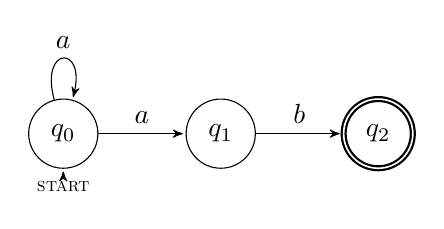
\begin{tikzpicture}[>=stealth',shorten >=1pt,auto,node distance=2cm]
		\node[state, initial]   (q0)                 {$q_0$};
		\node[state]            (q1) [right of = q0] {$q_1$};
		\node[state, accepting] (q2) [right of = q1] {$q_2$};

		\path[->] (q0) edge [loop above] node {$a$} (q0);
		\path[->] (q0) edge              node {$a$} (q1);
		\path[->] (q1) edge              node {$b$} (q2);
	\end{tikzpicture}
	\end{center}
	\pause
	Accepts $ab, \, aab, \, aaab, \dots$.
\end{frame}
\note[itemize]{
	\item All the automata we've dealt with so far have exactly one transition from each state on each input, but this is not actually required.
	Automata with this restriction are DFAs.
	\item We can build automata without this restriction: they are called nondeterministic, abbreviated to NDFA.
	\item This automaton has two transitions from $q_0$ on $a$, to itself and to $q_1$. 
			There is no transition from $q_1$ on $a$, and no transition from $q_0$ on $b$.
	\item Talk about how it behaves.
}

\begin{frame}
	\frametitle{NDFAs are Tricky}
	We no longer have transitions to a single state.
	\[
		\delta : (Q \times \Sigma) \to 2^Q
	\]
	($2^Q$ is the set of all subsets of $Q$)\\[2 ex]

	\pause
	We write
	\[
		q_1 \in \delta(q_0, a) %\quad \text{ or } \quad q_1 \in \Delta(q_0, a)
	\]
	instead of 
	\[
		\delta(q_0, a) = q_1 %\quad \text{ or } \quad \Delta(q_0, a) = q_1
	\]

\end{frame}
\note[itemize]{
	\item any subset of the states may be active at once, so we need define transitions to the power set of $Q$.
	\item We say that a state is IN the result of the transition, rather than EQUAL to the result of the transition.
}

\begin{frame}
	\frametitle{Kleene's Theorem}
	A language is represented by a finite automaton if and only if it is regular.

	\begin{enumerate}
		\pause
		\item All regular languages are represented by an NDFA.
		\pause
		\item A language is representable by an NDFA if and only if it is representable by a DFA.
		\pause
		\item All representable languages are regular.
	\end{enumerate}
\end{frame}

\begin{frame}
	\frametitle{The Atomic Regular Languages are Representable}
	\begin{figure}[H]
		\centering
		\visible<1->{
			\begin{subfigure}[b]{0.3 \textwidth}
				\centering
				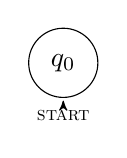
\begin{tikzpicture}[>=stealth',shorten >=1pt,auto,node distance=2cm]
					\node[initial,state] (q0)                {$q_0$};
				\end{tikzpicture}
				\caption*{Accepts $\emptyset$}
			\end{subfigure}
		}
		\visible<2->{
			\begin{subfigure}[b]{0.3 \textwidth}
				\centering
				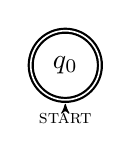
\begin{tikzpicture}[>=stealth',shorten >=1pt,auto,node distance=2cm]
					\node[initial,state, accepting] (q0)                {$q_0$};
				\end{tikzpicture}
				\caption*{Accepts $\{ \lambda \}$}
			\end{subfigure}
		}
		\visible<3->{
			\begin{subfigure}[b]{0.3 \textwidth}
				\centering
				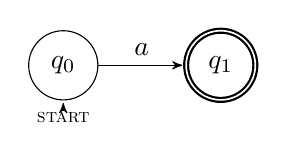
\begin{tikzpicture}[>=stealth',shorten >=1pt,auto,node distance=2cm]
					\node[initial,state]    (q0)                 {$q_0$};
					\node[state, accepting] (q1) [right of = q0] {$q_1$};
					\path[->](q0) edge  node {$a$} (q1);
				\end{tikzpicture}
				\caption*{Accepts $\{ a \}$}
			\end{subfigure}
		}
	\end{figure}
\end{frame}
\note[itemize]{
	\item We first show that all the atomic regular languages are representable by constructing NDFAs to represent them.
	\item Then we construct automata for regular combinations
	\item It's easy to construct a machine that represent the empty set --- it just has to accept no strings at all.
	\item To accept just the empty string, we have an initial state that is accepting, and define no transitions. 
	(implicit is no transition means transition to dead state.)
	\item This should make the difference between the empty set and the empty string clear.
	\item Finally, single symbol.
}

\begin{frame}
	\frametitle{Combining Representable Languages}
	\begin{figure}[H]
		\begin{subfigure}{0.5 \textwidth}
			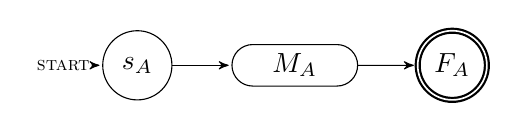
\begin{tikzpicture}[>=stealth',shorten >=1pt,auto,node distance=2cm, initial left]
				\node[initial,state]    (q0)                   {$s_A$};
				\node[elliptic state]   (ma)  [right of  = q0] {$\quad M_A \quad$};
				\node[state, accepting] (fa)  [right of = ma]  {$F_A$};
				\path[->](q0) edge (ma);
				\path[->](ma) edge (fa);
			\end{tikzpicture}
		\end{subfigure}\\[2 em]
		\begin{subfigure}{0.5 \textwidth}
			\begin{tikzpicture}[>=stealth',shorten >=1pt,auto,node distance=2cm, initial left]
				\node[initial,state]    (q0)                   {$s_B$};
				\node[elliptic state]   (mb)  [right of  = q0] {$\quad M_B \quad$};
				\node[state, accepting] (fb)  [right of = ma]  {$F_B$};
				\path[->](q0) edge (mb);
				\path[->](mb) edge (fb);
			\end{tikzpicture}
		\end{subfigure}
	\end{figure}
\end{frame}
\note{
	If languages are representable we have machines that represent them.
	So we can combine these machines to represent combinations of the languages.\\[2 ex]

	Introduce my rough diagrams.
	Mention that the sets of states are not shown with perfect accuracy.

}

\begin{frame}
	\frametitle{Union of Representable Languages}
	\begin{figure}[H]
		\centering
		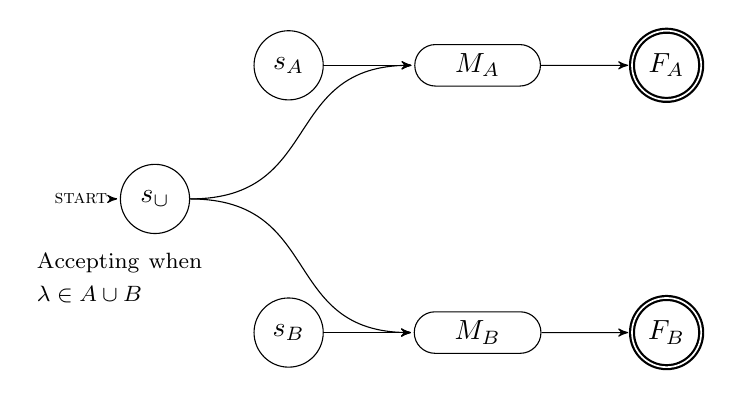
\begin{tikzpicture}[>=stealth',shorten >=1pt,auto,node distance=2.4cm, initial left]
			\visible<2->{
				\node[initial,state]    (sab)                             {$s_\cup$};
			}

			\visible<1->{
				\node[state]            (sa)  [above right of = sab]      {$s_A$};
				\node[elliptic state]   (ma)  [right of = sa]             {$\quad M_A \quad$};
				\node[state,accepting]  (fa)  [right of = ma]             {$F_A$};
				\path[->](sa) edge (ma);
				\path[->](ma) edge (fa);

				\node[state]            (sb)  [below right of = sab]      {$s_B$};
				\node[elliptic state]   (mb)  [right of = sb]             {$\quad M_B \quad$};
				\node[state, accepting] (fb)  [right of = mb]             {$F_B$};
				\path[->](sb) edge (mb);
				\path[->](mb) edge (fb);
			}
			\visible<3->{
				\path[->](sab) edge [out=0, in=180, distance = 1.7 cm] (ma);
				\path[->](sab) edge [out=0, in=180, distance = 1.7 cm] (mb);
			}
			\visible<4->{
				\node  (sab_label)   [below of = sab,node distance=1cm, text width=3cm] {\footnotesize{Accepting when\\$\lambda \in A \cup B$}};
			}
		\end{tikzpicture}
	\end{figure}
\end{frame}

\begin{frame}
	\frametitle{Concatenation of Representable languages}
	
\end{frame}



\begin{frame}[shrink]
	\frametitle{References}
	\bibliographystyle{amsplain}
	\nocite{*}
	\bibliography{../paper/references.bib}
\end{frame}

\end{document}
